% Setup  %
\documentclass[12pt,letterpaper]{article}
\usepackage{graphicx,textcomp}
\usepackage{natbib}
\usepackage{setspace}
\usepackage{fullpage}
\usepackage{color}
\usepackage[reqno]{amsmath}
\usepackage{amsthm}
\usepackage{fancyvrb}
\usepackage{amssymb,enumerate}
\usepackage[all]{xy}
\usepackage{endnotes}
\usepackage{lscape}
\newtheorem{com}{Comment}
\usepackage{float}
\usepackage{hyperref}
\newtheorem{lem} {Lemma}
\newtheorem{prop}{Proposition}
\newtheorem{thm}{Theorem}
\newtheorem{defn}{Definition}
\newtheorem{cor}{Corollary}
\newtheorem{obs}{Observation}
\usepackage[compact]{titlesec}
\usepackage{dcolumn}
\usepackage{tikz}
\usetikzlibrary{arrows}
\usepackage{multirow}
\usepackage{xcolor}
\usepackage{fancyvrb}
\newcolumntype{.}{D{.}{.}{-1}}
\newcolumntype{d}[1]{D{.}{.}{#1}}
\definecolor{light-gray}{gray}{0.65}
\usepackage{url}
\usepackage{listings}
\usepackage{color}
\usepackage{etoolbox}
\usepackage{tabularx}
\makeatletter
\preto{\@verbatim}{\topsep=0pt \partopsep=0pt }
\makeatother
\usepackage{placeins}
\usepackage{listings}
\usepackage[utf8]{inputenc}
\usepackage[T1]{fontenc}
\usepackage{pdfpages}

\definecolor{codegreen}{rgb}{0,0.6,0}
\definecolor{codegray}{rgb}{0.5,0.5,0.5}
\definecolor{codepurple}{rgb}{0.58,0,0.82}
\definecolor{backcolour}{rgb}{0.95,0.95,0.92}

\lstdefinestyle{mystyle}{
	backgroundcolor=\color{backcolour},   
	commentstyle=\color{codegreen},
	keywordstyle=\color{magenta},
	numberstyle=\tiny\color{codegray},
	stringstyle=\color{codepurple},
	basicstyle=\footnotesize,
	breakatwhitespace=false,         
	breaklines=true,                 
	captionpos=b,                    
	keepspaces=true,                 
	numbers=left,                    
	numbersep=5pt,                  
	showspaces=false,                
	showstringspaces=false,
	showtabs=false,                  
	tabsize=2
}
\lstset{style=mystyle}
\newcommand{\Sref}[1]{Section~\ref{#1}}
\newtheorem{hyp}{Hypothesis}

\title{Data Visualisation for Social Scientists -  Final Project}
\date{Due: March 8, 2026}
\author{Ellen Beattie}

\begin{document}
	\maketitle
	
\tableofcontents
\vspace*{1cm}
	
\section{Executive Summary}
This project aims to investigate how the United Kingdom measures up in the development and integration of Artificial Intelligence (AI). Through the use of visualisations I will explore how the UK compares to other countries on the world stage, specifically in terms of economic development, public opinion and ethical/responsible practices and governance. By visualising the data I aim to gain key insights into the topic and capture a snapshot of the current state of the UK with regards to AI.


\section{Data Background}

The data used in this project is from the a Global Artificial Intelligence Indicator Database (GAID) 1998-2025, sourced from the \href{https://dataverse.harvard.edu/dataset.xhtml?persistentId=doi:10.7910/DVN/QYLYSA}{Harvard Dataverse}. This longitudinal panel dataset sources, standardises and consolidates indicator information from Stanford's AI Index, OECD.ai and the Global Index on Responsible AI (GIRAI). It contains information from 214 countries, across 28 years with data on 24,323 unique metrics. There is varying levels of coverage across the data, and the metrics are grouped into key source categories such as Economy, Education, Public Opinion etc. There is a comprehensive codebook accessible with detailed descriptions of the topics, specific metrics and the units of measurement. 


\section{Data Cleaning}

After downloading and importing the CSV file, I explored the underlying data structure. The data was provided in long form, making it easier to filter and clean for plotting each individual figure. Packages were loaded along with the data.  
	\lstinputlisting[language=R, firstline=26, lastline= 30]{Final_Project_EB.R}  
	\lstinputlisting[language=R, firstline=79, lastline= 81]{Final_Project_EB.R} 
	
For simplicity and consistency I created a base theme to apply to all the figures, as well as a base colour palette. 
	\lstinputlisting[language=R, firstline=36, lastline= 75]{Final_Project_EB.R} 



\section{Individual Figures}
\vspace{1cm}
\subsection{Figure 1: Plot of AI Vibrancy Scores Economy vs R{\&}D}

First, I wanted to understand the landscape of global AI development. To do this I created Figure 1 which plots the relative positions of major world countries on two axes: Research and Development describing the countries' AI innovation capacity including components such as AI journal/conference publications and AI-related patent fillings/grants; and Economic describing the countries' capacity to exploit AI including talent intensity, investment, new AI companies and AI skill penetration. The normalised vibrancy score on these two dimension is sourced from the Stanford Global Vibrancy index.   \\

\lstinputlisting[language=R, firstline=84, lastline= 120]{Final_Project_EB.R} 

\begin{figure}[!htbp]\centering
	\label{fig:plot_1}
	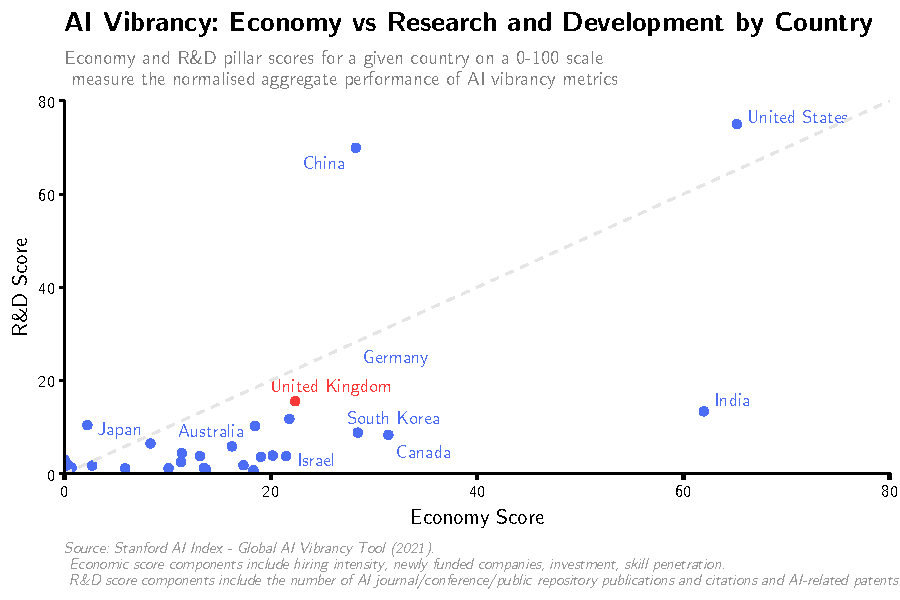
\includegraphics[width=0.95\linewidth]{figures/figure1.pdf}
\end{figure}
\FloatBarrier

Figure 1 shows that the US, China and India are clear outliers in different ways. The US has a leadership position in both dimensions, whereas China appears to be less able to capitalise economically on its strong capability in AI R\&D. Conversely, India is well-positioned to economically exploit AI but is less productive in terms of innovation measures. Within the chasing pack the UK ranks third in R\&D but sixth in economic development. Generally most other countries appear to perform better on economic metrics than on R\&D.

\vspace{1cm}
\subsection{Figure 2: Bar Chart of Total Private Investment in AI}

To better understand the level of private investment in AI, I analysed the level of private capital investment per country over the last twelve years. Figure 2 shows a bar chart of the cumulative amount of investment (2013-2024) of the top countries in the world, highlighting the UK by colour and adding the value (in billions USD) to each bar to easily display the total private capital invested in each country. \\ 

	\lstinputlisting[language=R, firstline=129, lastline= 162]{Final_Project_EB.R} 

	\begin{figure}[!htbp]\centering
		\label{fig:plot_2}
		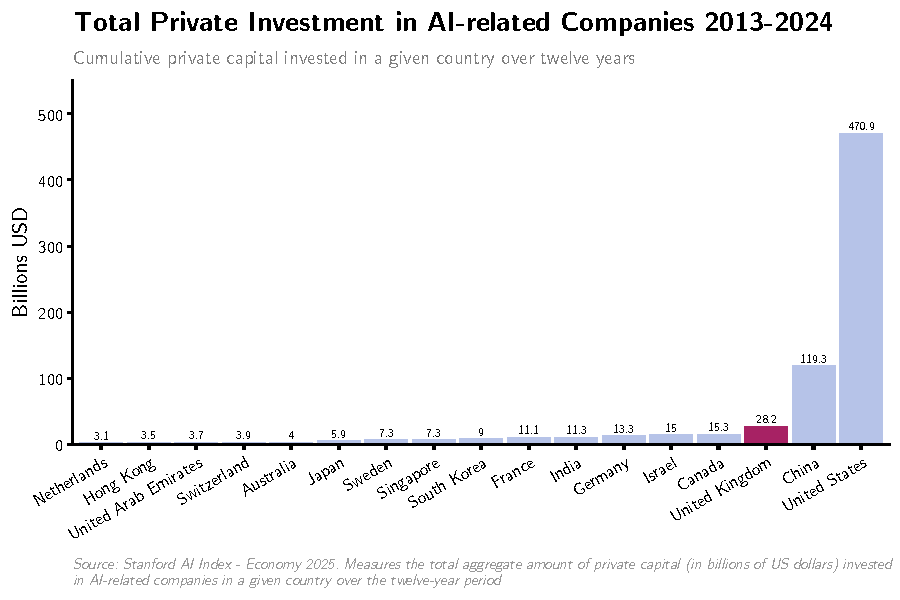
\includegraphics[width=0.95\linewidth]{figures/figure2.pdf}
	\end{figure}
	\FloatBarrier
	
Figure 2 shows how much more the US (and to some degree China) has invested privately in AI compared to the rest of the world. The UK was surprisingly high relative to other comparable countries, coming in third globally with 28.2 billion dollars of investment being recorded between 2013 and 2024. This suggests that people have determined that AI companies in the UK are worth investing in and may be profitable, managing to gain more investment than any other European nations of similar size.


\vspace{1cm}
\subsection{Figure 3: Percentage Stacked Bar Chart of Female AI Talent Representation }

I wanted to look further into the UK's AI capabilities, and in particular at the workforce composition and whether AI talent is spread across genders. To do this I plotted a percentage stacked bar chart to easily visualise what proportion of AI specialists identified as female versus male. By lining up the countries it is easy to determine how much different workforces differ in terms of gender representation and how the UK compares.\\

\lstinputlisting[language=R, firstline=170, lastline= 218]{Final_Project_EB.R} 

\begin{figure}[!htbp]\centering
	\label{fig:plot_3}
	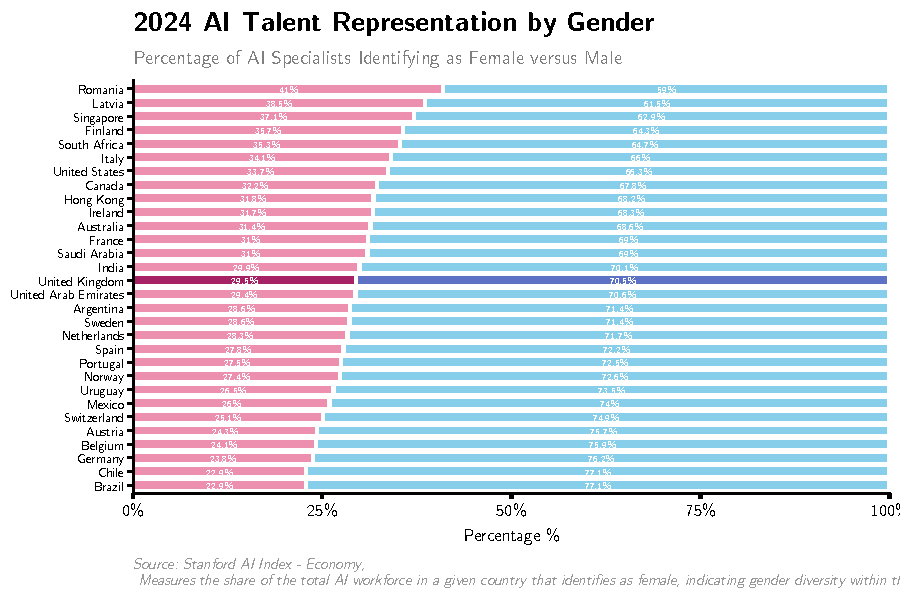
\includegraphics[width=0.95\linewidth]{figures/figure3.pdf}
\end{figure}
\FloatBarrier

Figure 3 shows that, globally, women are under-represented within the AI-talent workforce.  
The UK in 2024 appeared solidly in the middle of the pack in terms of female talent representation with 29.5\% female to 70.5\% male. The US is higher by about 5\% whereas Germany, Chile and Brazil have the lowest representation with less than a quarter of their AI talent being female. Interestingly there does not appear to be a clear trend in nation location, investment and gender equality, but it is concerning to see the gender disparity in a sector that is projected to have massive implications for the economy. For the UK specifically, given the high level of overall investment, the country might consider what advantage it could gain by investing in female AI talent. 


\vspace{1cm}
\subsection{Figure 4: Bar Chart of Public Opinion Impact of AI on Daily Life in the Past and Future}

Moving beyond these economic and R\&D factors, I was also interested in understanding how the UK public think and feel about AI. Firstly I created a bar chart using the Stanford Public Opinion index based on survey data that describes whether people feel that AI has profoundly changed their life in the past 3-5 years and their projections about whether it will in the next 3-5 years.  As the metric from the survey refers to the percentage that agree with a specific statement, and as in all cases there was a higher percentage agreeing on future impact,  a dodged bar chart was used. This allows both percentages to be plotted together for each country allowing for easy comparison of each between countries as well as the size of the difference between the two metrics. \\

\lstinputlisting[language=R, firstline=223, lastline= 277]{Final_Project_EB.R} 

\begin{figure}[!htbp]\centering
	\label{fig:plot_4}
	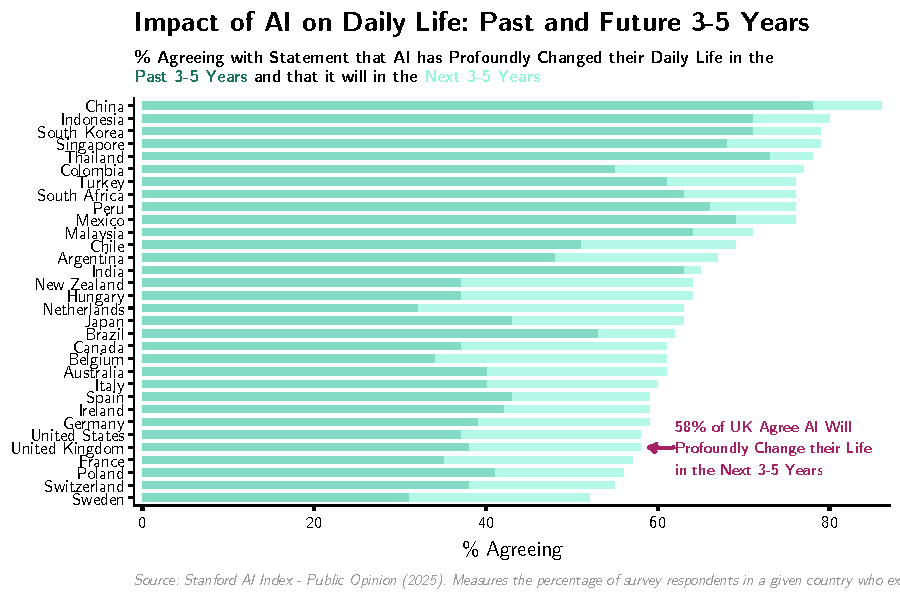
\includegraphics[width=0.95\linewidth]{figures/figure4.pdf}
\end{figure}
\FloatBarrier


Figure 4 highlights that people in the UK feel like their lives have been, and will continue to be, less impacted by AI than other countries.This is in stark contrast to China and other Asian countries where the public reports  very high levels of change due to AI in the past 3-5 years (over 70\%) and with even more people believing it will in the future (in China over 80\% of those surveyed). Interestingly, the US and other European nations appear to be in a  similar position to the UK, with a much lower proportion of people reporting a profound change in their daily lives due to AI so far. In all these countries a higher number of people (typically 20\% more) believe that AI will cause profound change in daily lives in the next 3-5 years .

\vspace{1cm}
\subsection{Figure 5: Excited or Nervous? Lollipop Chart of Public Emotion on AI}

As well as reported and expected impact of AI, I was also interested in public emotion about AI, so I analysed the opinion index on the percentage of people that feel excited or nervous about products and services that use AI in each country. Unlike the previous Figure, there was a clear split between countries where people wer more excited than nervous, and vice versa. To visualise this clearly I decided to use a lollipop chart where points correspond to the specific emotion (excited or nervous) and the distance between the two represented by a line connection. \\

\lstinputlisting[language=R, firstline=286, lastline= 339]{Final_Project_EB.R} 

\begin{figure}[!htbp]\centering
	\label{fig:plot_5}
	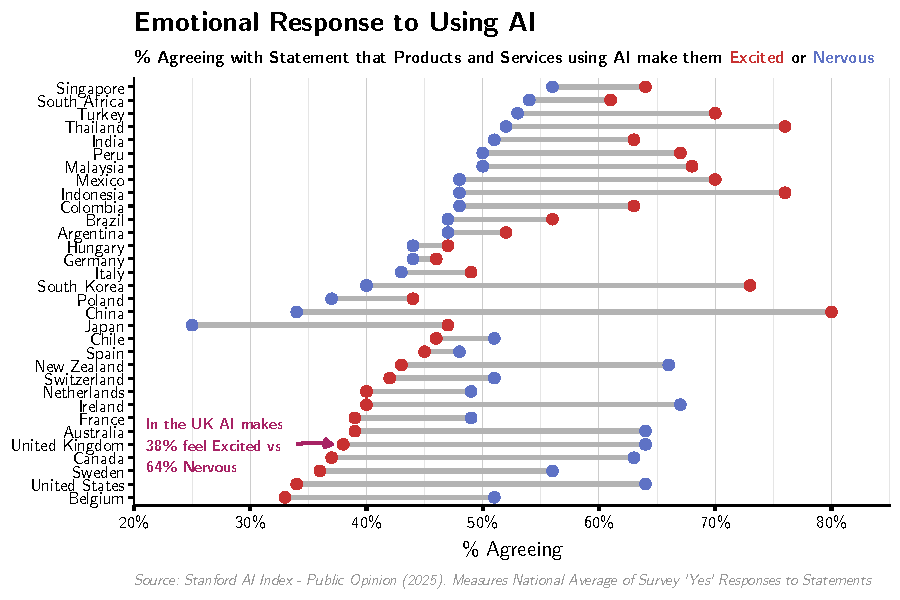
\includegraphics[width=0.95\linewidth]{figures/figure5.pdf}
\end{figure}
\FloatBarrier


Figure 5 shows a large cohort of countries where more people agreeing with the statement they feel excited about AI product than nervous, whilst another cohort where people feel more nervous than excited (some potentially feeling both). Countries on the top half of the chart fall in the first group, comprising mainly Asian and South American countries, whilst the latter group is primarily European and North American countries, including the UK. \\
 In the UK 64\% agree that they feel nervous and 38\% feel excited, indicating that generally the UK public is apprehensive about the prospect of AI. The difference between the UK and China is remarkable, with $>$40\% difference in people feeling excited and a $>$30\% difference in people feeling nervous. There does not appear to be a clear link between economic and R\&D capacity (Figure 1) and subsequent public sentiment about AI, indicating other factors likely contribute to emotions regarding AI. 


\vspace{1cm}

\subsection{Figure 6: Map of Global Responsible AI Index Score }

Finally, I wanted to look into how the UK performs on metrics reporting ethical use of AI particularly how responsible the UK practices and governance is on ensuring human rights are maintained.   
Initially I was intrigued whether there are any interesting global patterns in the countries that are more concerned at pursuing AI in a responsible manner, and the performance of the UK in particular. Using the GIRAI Index Score for each country in 2024, I visualised this score on a world map, pairing the colour to the index score to show patterns in country location more clearly.  \\

\lstinputlisting[language=R, firstline=344, lastline= 388]{Final_Project_EB.R} 

\begin{figure}[!htbp]\centering
	\label{fig:plot_6}
	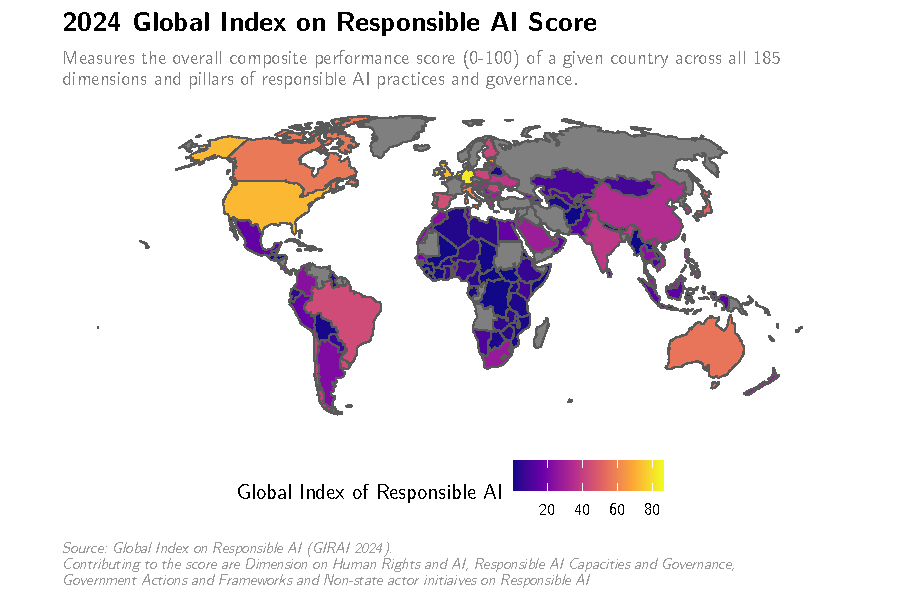
\includegraphics[width=0.95\linewidth]{figures/figure6.pdf}
\end{figure}
\FloatBarrier


Figure 6 maps countries using the Global Index of Responsible AI, showing that Western nations including the UK are the most responsible in term of AI practice. The UK appears to be at the top end of this score index, on par with the US but behind Germany and the Netherlands.  Other countries like Canada, Japan, Australia follow, with China and India scoring around 40 points. Lower levels of responsible practices and governance are seen in South East Asia, South Central America and Africa. This illustrates that the UK is performing well on Responsible AI metrics with room for improvement. 


\vspace{1cm}
\subsection{Figure 7: Scatter plot of Human Right Score and Trust in AI to not discriminate}

Finally, I wanted to explore the relationship between a country's Human Rights with regard to AI and  public trust in AI being non-discriminatory. Plotting each country by their GIRAI Dimension score on Human Rights  visualises the extent to which they takes steps to protect, promote, and respect human rights implicated by AI such as privacy, equality, and freedom; and the public opinion section of Stanford's AI index as the percentage of individuals that say they trust AI to not discriminate or bias towards any groups. \\

\lstinputlisting[language=R, firstline=392, lastline= 431]{Final_Project_EB.R} 

\begin{figure}[!htbp]\centering
	\label{fig:plot_7}
	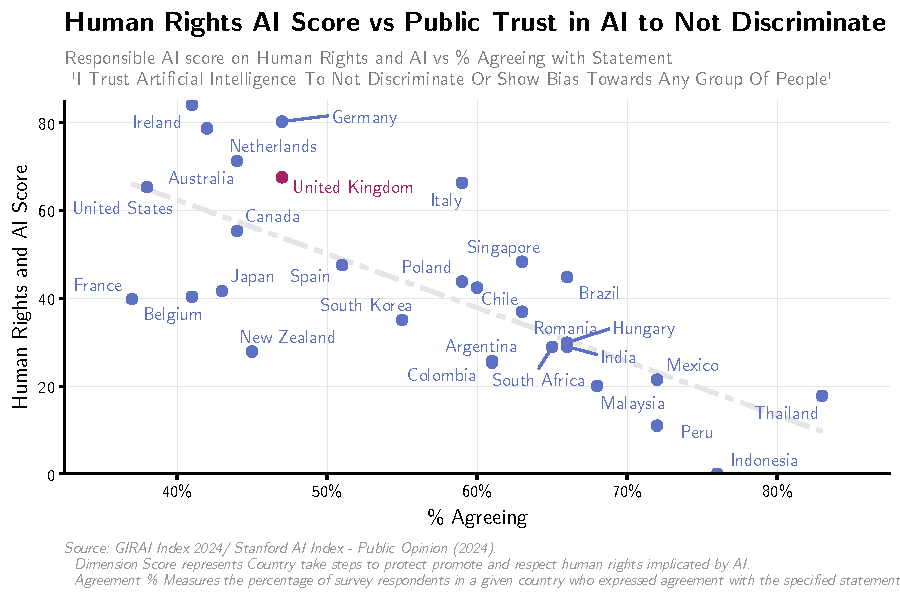
\includegraphics[width=0.95\linewidth]{figures/figure7.pdf}
\end{figure}
\FloatBarrier

Figure 7 shows that there is a surprising negative relationship between a country's Human Rights score and Trust in AI not to discriminate, i.e. countries with a level of trust tend to rate lower on the human right score. 
The UK has a moderately high Human Rights and AI score (>60) yet a less then half of the public surveyed said that they trusted AI to not discriminate or show bias. This may indicate that countries in which greater efforts are made to set up frameworks resulting in the public becoming more aware of the risk of AI being discriminatory. Alternatively it may also be that countries with low levels of public trust in AI put in greater Human Rights Frameworks.  A deeper investigation would be necessary to further understand this trend. 



\vspace{1cm}
\section{Final Figure}
Final Figure was compiled on separate txt file and uploaded as a final pdf.
\newpage
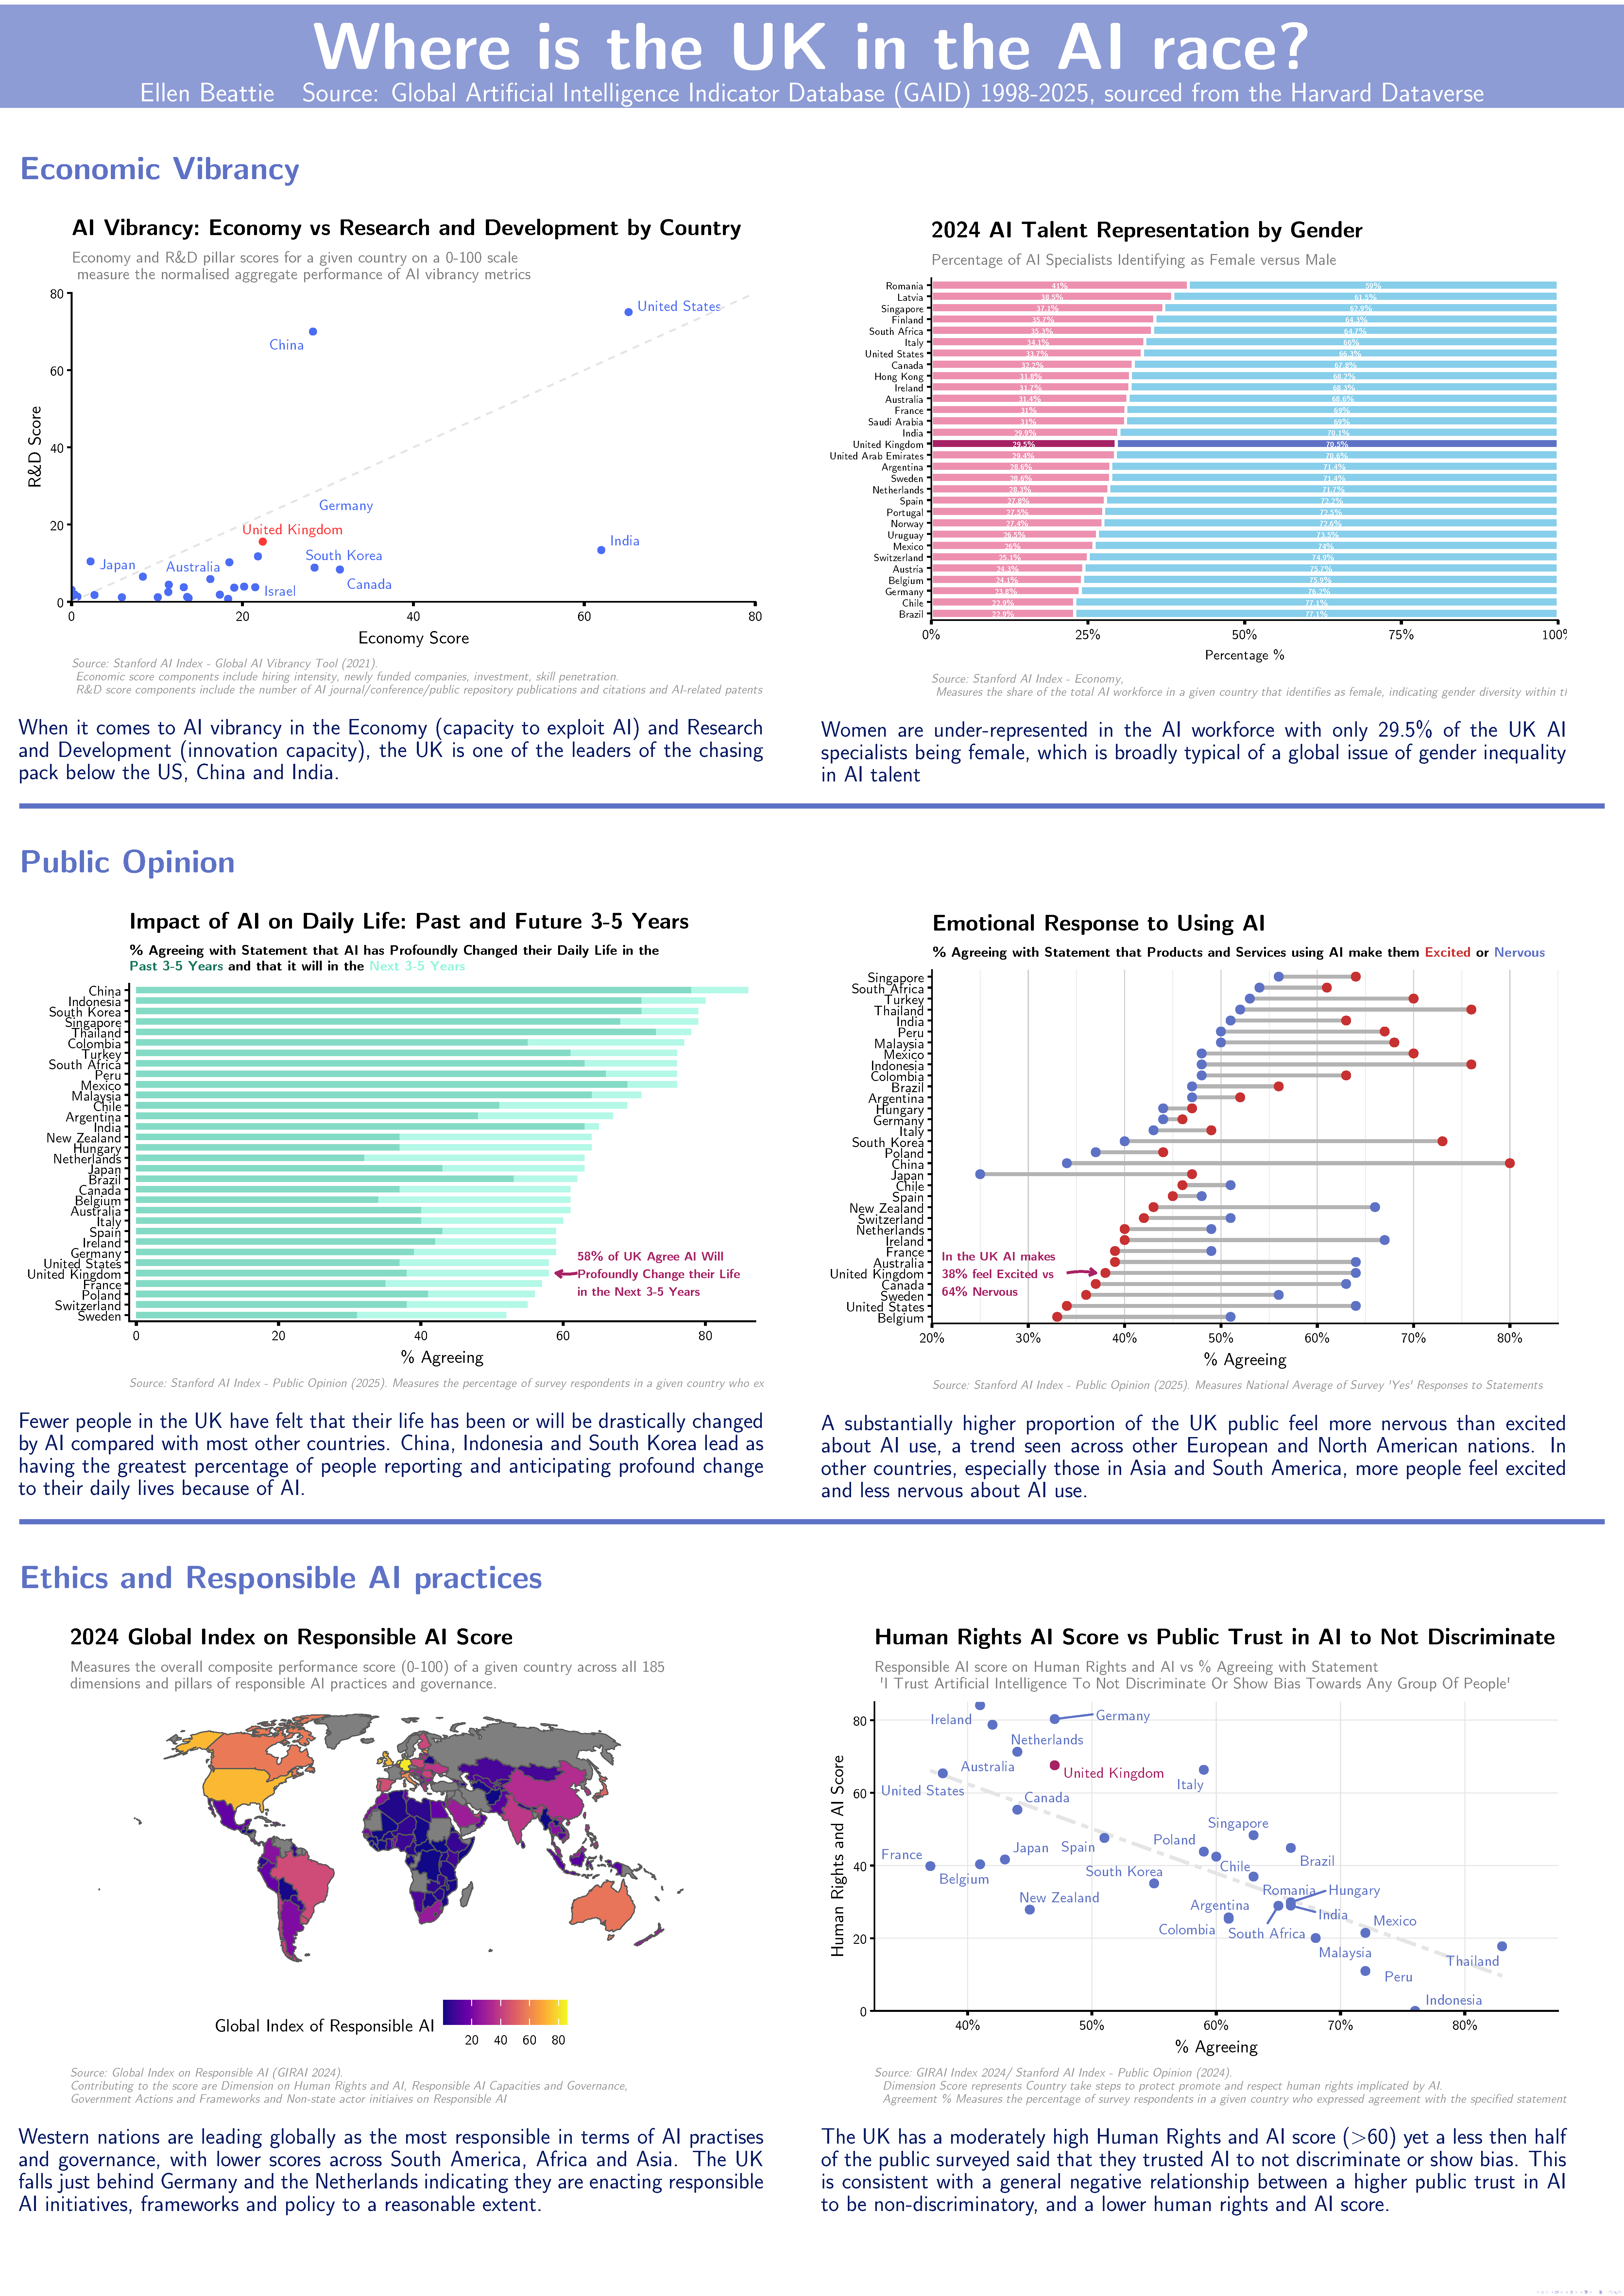
\includepdf[pages=-]{Final_Figure.pdf}

	

\end{document}
